\documentclass[Naxsi]{subfiles}
\begin{document}
\section{Naxsi}
\label{sec:Naxsi}
Naxsi is written to be a fast, light and scalable \ac{WAF} for the Nginx web server. Naxsi means Nginx Anti Xss \& Sql Injection and it has a positive approach for web traffic inspection by using a white listing method. This means that traffic is blocked by default, and "good" traffic must be explicitly allowed. Naxsi uses two different files, which contain the rules. First, at the server level configuration. Second, at the HTTP location level configuration. The first one is called the \emph{core rules}, and it contains all characters and regular expressions that will increase the score of the request when the request has invalid content. The location level configuration has site specific rules and, thus allows for multiple virtual hosts. The local level configuration allows for each site to specify when a request should be dropped depending on the score the request is given by Naxsi.\\
The core level configuration can be referred to as blacklist. Furthermore it is more or less a fixed list and, according to the Nginx website~\footnote{\url{https://code.google.com/p/naxsi/wiki/HowDoesItWork}}, it is not expected to evolve rapidly. On the other hand, the local level configuration is a site specific configuration, and thus needs to be created. Creating the rules is done by putting Naxsi in learning mode. When Naxsi is in learning mode, no request will be blocked, but rather it is seen as valid traffic and used for creating the whitelist rule set.

\subsection{Request flow}
When Naxsi is in production mode, it will actively give each request a score. Depending on the local level configuration rule set, the request may be allowed or dropped. Figure \ref{fig:naxsi_flow} shows how logically each request is processed by Naxsi. First, the request is checked for "dangerous" symbols and SQL keywords. Second, the request is checked by the local level rules. Local level rules may overrule the core rules if configured such. Lastly, the request score is checked against the rule set. Depending on the score, the request is either blocked, which means the request gets forwarded to the DeniedURL, or the request is further processed.

\begin{figure}[h]
\caption{Naxsi request flow}
\centering
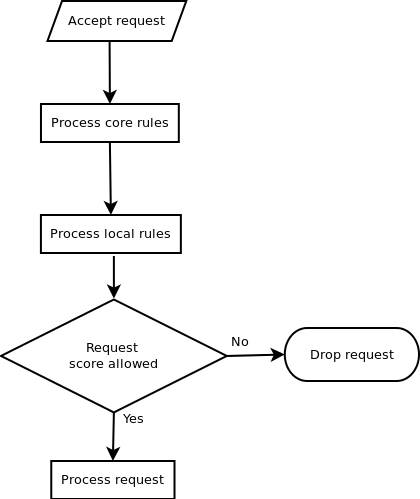
\includegraphics[width=0.5\textwidth] {images/naxsi_flow.png}
\label{fig:naxsi_flow}
\end{figure}

\subsection{Whitelist processing}
\label{sec:naxsi_whitelist}
As discussed before Naxsi does have a short blacklist. However, the usage of whitelists is more extensive. This is why some more attentions is brought to the details of processing hereof.

Upon startup of Naxsi the local rules file(s) are read and hashtables for the so called zones are created in memory (see fig.~\ref{fig:hashtables}). The zones are respectively:
\begin{itemize}
	\item ARGS (GET arguments)
	\item URL (the full URI)
	\item BODY (POST arguments)
	\item HEADER (HTTP headers)
\end{itemize}

Once a HTTP request is accepted, it is parsed and split up into 4 streams: ARGS, URL, BODY, HEADERS. Each stream, that may consist of more parameters, is iterated through independently, but in the same manner. Each parameter is checked for suspicious patterns. The core rules are consulted as to whether it contains "dangerous" symbols. Furthermore a lookup in the respective zone hashtable (as created during startup, see fig.~\ref{fig:hashtables}) is done, as to determine whether this specific match has been whitelisted. If it has \emph{not} been whitelisted the score that is attached to the matching core rule is applied. When all streams are iterated through, eventually it is determined if the summed up score for  (SQL, RFI, TRAVERSAL, XSS) is below the threshold. If it is, the REQUEST is forwarded. If not, it is dropped. 

\begin{figure}[h]
\caption{Creating hashtables from local rules}
\centering
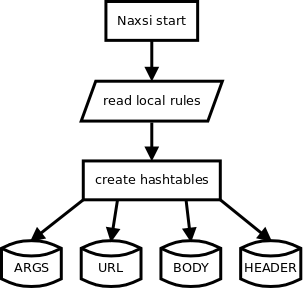
\includegraphics[width=0.5\textwidth] {images/hashtables.png}
\label{fig:hashtables}
\end{figure}

This approach shows that matching is done very efficient. Creating hashtables from the rules, should fasten the process of lookups. Furthermore through splitting up the REQUEST data in the same manner as the hashtables, the processing of parameters is handled separate and thereby effectively.

\begin{figure}[h]
\caption{Naxsi whitelist processing}
\centering
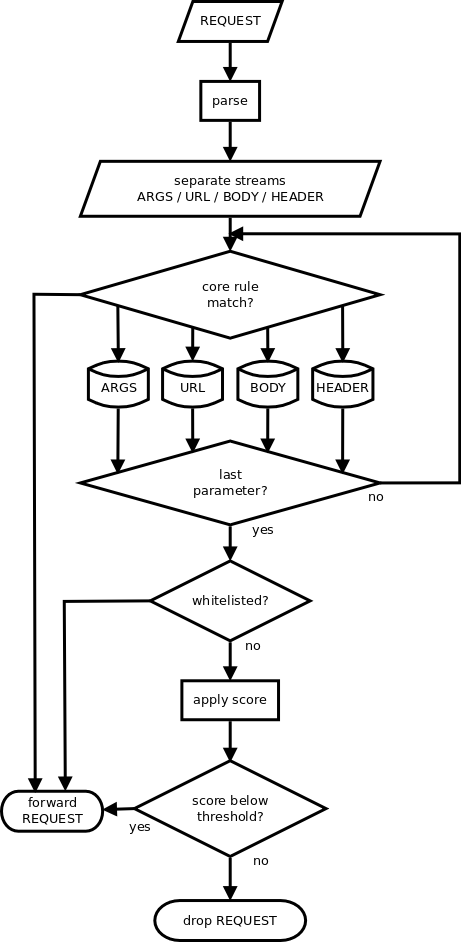
\includegraphics[width=0.5\textwidth] {images/whitelist_processing.png}
\label{fig:whitelist_processing}
\end{figure}



\end{document}

